\documentclass[12pt,twoside]{article}
%%%%%%%%%%%%%%%%%%%%%%%%%%%%%%%%%%%%%%%%%%%%%%%%%%%%%%%%%%%%%
% Meta informations:
\newcommand{\trauthor}{Sayantan Auddy}
\newcommand{\trtype}{Seminar Paper} %{Seminararbeit} %{Proseminararbeit}
\newcommand{\trcourse}{Independent Study}
\newcommand{\trtitle}{Biped Locomotion using Central Pattern Generators}
\newcommand{\trmatrikelnummer}{6640595}
\newcommand{\tremail}{4auddy@informatik.uni-hamburg.de}
\newcommand{\trarbeitsbereich}{Knowledge Technology, WTM}
\newcommand{\trdate}{03.11.2016}

%%%%%%%%%%%%%%%%%%%%%%%%%%%%%%%%%%%%%%%%%%%%%%%%%%%%%%%%%%%%%
% Languages:

% Falls die Ausarbeitung in Deutsch erfolgt:
% \usepackage[german]{babel}
% \usepackage[T1]{fontenc}
% \usepackage[latin1]{inputenc}
% \usepackage[latin9]{inputenc}	 				
% \selectlanguage{german}

% If the thesis is written in English:
\usepackage[english]{babel} 						
\selectlanguage{english}

%%%%%%%%%%%%%%%%%%%%%%%%%%%%%%%%%%%%%%%%%%%%%%%%%%%%%%%%%%%%%
% Bind packages:
\usepackage{acronym}                    % Acronyms
\usepackage{algorithmic}				% Algorithms and Pseudocode
\usepackage{algorithm}					% Algorithms and Pseudocode
\usepackage{amsfonts}                   % AMS Math Packet (Fonts)
\usepackage{amsmath}                    % AMS Math Packet
\usepackage{amssymb}                    % Additional mathematical symbols
\usepackage{amsthm}
\usepackage{booktabs}                   % Nicer tables
%\usepackage[font=small,labelfont=bf]{caption} % Numbered captions for figures

\usepackage{color}                      % Enables defining of colors via \definecolor
\definecolor{uhhRed}{RGB}{254,0,0}      % Official Uni Hamburg Red
\definecolor{uhhGrey}{RGB}{122,122,120} % Official Uni Hamburg Grey
\usepackage{fancybox}                   % Gleichungen einrahmen
\usepackage{fancyhdr}					% Packet for nicer headers
%\usepackage{fancyheadings}             % Nicer numbering of headlines

%\usepackage[outer=3.35cm]{geometry} 	% Type area (size, margins...) !!!Release version
%\usepackage[outer=2.5cm]{geometry} 	% Type area (size, margins...) !!!Print version
%\usepackage{geometry} 					% Type area (size, margins...) !!!Proofread version
\usepackage[outer=3.15cm]{geometry} 	% Type area (size, margins...) !!!Draft version
\geometry{a4paper,body={5.8in,9in}}

\usepackage{graphicx}                   % Inclusion of graphics
%\usepackage{latexsym}                  % Special symbols
\usepackage{longtable}					% Allow tables over several pages
\usepackage{listings}                   % Nicer source code listings
\usepackage{multicol}					% Content of a table over several columns
\usepackage{multirow}					% Content of a table over several rows
\usepackage{rotating}					% Alows to rotate text and objects
\usepackage[hang]{subfigure}            % Allows to use multiple (partial) figures in a fig
%\usepackage[font=footnotesize,labelfont=rm]{subfig}	% Pictures in a floating environment
\usepackage{tabularx}					% Tables with fixed width but variable rows
\usepackage{url,xspace,boxedminipage}   % Accurate display of URLs
\usepackage{multirow}
\usepackage{tabulary}
\usepackage{float}
%%%%%%%%%%%%%%%%%%%%%%%%%%%%%%%%%%%%%%%%%%%%%%%%%%%%%%%%%%%%%
% Configurationen:

\hyphenation{whe-ther} 					% Manually use: "\-" in a word: Staats\-ver\-trag

%\lstloadlanguages{C}                   % Set the default language for listings
\DeclareGraphicsExtensions{.pdf,.svg,.jpg,.png,.eps} % first try pdf, then eps, png and jpg
\graphicspath{{./src/}} 				% Path to a folder where all pictures are located
\pagestyle{fancy} 						% Use nicer header and footer

% Redefine the environments for floating objects:
\setcounter{topnumber}{3}
\setcounter{bottomnumber}{2}
\setcounter{totalnumber}{4}
\renewcommand{\topfraction}{0.9} 		%Standard: 0.7
\renewcommand{\bottomfraction}{0.5}		%Standard: 0.3
\renewcommand{\textfraction}{0.1}		%Standard: 0.2
\renewcommand{\floatpagefraction}{0.8} 	%Standard: 0.5

% Tables with a nicer padding:
\renewcommand{\arraystretch}{1.2}

%%%%%%%%%%%%%%%%%%%%%%%%%%%%
% Additional 'theorem' and 'definition' blocks:
\theoremstyle{plain}
\newtheorem{theorem}{Theorem}[section]
%\newtheorem{theorem}{Satz}[section]	% Wenn in Deutsch geschrieben wird.
\newtheorem{axiom}{Axiom}[section] 	
%\newtheorem{axiom}{Fakt}[chapter]		% Wenn in Deutsch geschrieben wird.
%Usage:%\begin{axiom}[optional description]%Main part%\end{fakt}

\theoremstyle{definition}
\newtheorem{definition}{Definition}[section]

%Additional types of axioms:
\newtheorem{lemma}[axiom]{Lemma}
\newtheorem{observation}[axiom]{Observation}

%Additional types of definitions:
\theoremstyle{remark}
%\newtheorem{remark}[definition]{Bemerkung} % Wenn in Deutsch geschrieben wird.
\newtheorem{remark}[definition]{Remark} 

%%%%%%%%%%%%%%%%%%%%%%%%%%%%
% Provides TODOs within the margin:
\newcommand{\TODO}[1]{\marginpar{\emph{\small{{\bf TODO: } #1}}}}

%%%%%%%%%%%%%%%%%%%%%%%%%%%%
% Abbreviations and mathematical symbols
\newcommand{\modd}{\text{ mod }}
\newcommand{\RS}{\mathbb{R}}
\newcommand{\NS}{\mathbb{N}}
\newcommand{\ZS}{\mathbb{Z}}
\newcommand{\dnormal}{\mathit{N}}
\newcommand{\duniform}{\mathit{U}}

\newcommand{\erdos}{Erd\H{o}s}
\newcommand{\renyi}{-R\'{e}nyi}
\setlength{\parindent}{0pt}
\newcommand{\forceindent}{\leavevmode{\parindent=2em\indent}}
%%%%%%%%%%%%%%%%%%%%%%%%%%%%%%%%%%%%%%%%%%%%%%%%%%%%%%%%%%%%%
% Document:
\begin{document}
\renewcommand{\headheight}{14.5pt}

\fancyhead{}
\fancyhead[LE]{ \slshape \trauthor}
\fancyhead[LO]{}
\fancyhead[RE]{}
\fancyhead[RO]{ \slshape \trtitle}

%%%%%%%%%%%%%%%%%%%%%%%%%%%%
% Cover Header:
\begin{titlepage}
	\begin{flushleft}
		Universit\"at Hamburg\\
		Department Informatik\\
		\trarbeitsbereich\\
	\end{flushleft}
	\vspace{3.5cm}
	\begin{center}
		\huge \trtitle\\
	\end{center}
	\vspace{3.5cm}
	\begin{center}
		\normalsize\trtype\\
		[0.2cm]
		\Large\trcourse\\
		[1.5cm]
		\Large \trauthor\\
		[0.2cm]
		\normalsize Matr.Nr. \trmatrikelnummer\\
		[0.2cm]
		\normalsize\tremail\\
		[1.5cm]
		\Large \trdate
	\end{center}
	\vfill
\end{titlepage}

	%backsite of cover sheet is empty!
\thispagestyle{empty}
\hspace{1cm}
\newpage

%%%%%%%%%%%%%%%%%%%%%%%%%%%%
% Abstract:

% Abstract gives a brief summary of the main points of a paper:
\section*{Abstract}
  

% Lists:
\setcounter{tocdepth}{2} 					% depth of the table of contents (for Seminars 2 is recommented)
\tableofcontents
\pagenumbering{arabic}
\clearpage

%%%%%%%%%%%%%%%%%%%%%%%%%%%%
% Content:

% the actual content, usually separated over a number of sections
% each section is assigned a label, in order to be able to put a
% crossreference to it

\graphicspath{{images/}}

\section{Introduction}
\label{sec:introduction}
\forceindent Walking on two feet is an activity that all of us take for granted. Yet this apparently simple action involves a host of complex mechanisms, both mechanical and neural, which are tied together to produce the efficient bipedal movements of human beings. The ability to move around on two legs has allowed humans to efficiently deal with a wide variety of terrains, be it flat grasslands or lush forests overrun by undergrowth or the concrete jungles which we now inhabit. Even from an evolutionary viewpoint, bipedal locomotion has enabled humans to move about while leaving their hands free to engage in more important tasks such as tool-making. The efficiency and versatility of biped movement is undeniable. It is only natural then, for us to desire our robots to have the same capabilities.\\ 
\forceindent While a vast majority of mobile robots today have wheels, the limitations of wheeled locomotion are obvious. Wheeled robots require a structured environment to operate in, and although certain types of wheeled robots can handle uneven terrain, their scope is still quite limited. Legged robots on the other hand can operate in much more diverse environments, and theoretically can handle any environment that humans can handle. As robots become more pervasive in society, the need for robots that can function in human environments will continue to grow. Even from a psychological perspective, anthropomorphic robots have the added advantage of being more acceptable to human users.\\
\forceindent However, the benefits of legged robots comes at a price. The challenges associated with bipedal movement are much more involved than those associated with wheeled locomotion. Bipedal locomotion is inherently unstable, and a considerable amount of effort goes into maintaining balance. The biped robot can be imagined as an inverted pendulum - even a small disturbance is enough to move it from its equilibrium position and unless corrective action is taken, the robot will topple over. In addition to this, bipedal locomotion is a complicated mix of the movements of different limbs in a synchronous fashion. Human walking involves multiple degrees of freedom and is achieved with the combined effort of muscles, bones, ligaments and tendons. Replicating this movement in robots using the conventional servo motors we have at our disposal today, is also a very difficult task.\\
\forceindent In the literature numerous approaches exist for solving the problem of bipedal locomotion. Perhaps the most popular approach is that of using the  Zero Moment Point (ZMP) introduced by Vukobratovic et al. in 1969 \cite{vukobratovic1969contribution, jurivcic1972mathematical}. In the decades since its inception, ZMP has been a popular choice for researchers around the world dealing with the problem of bipedal robots. ZMP is defined as that point on the ground at which the net moment of the inertial forces and the gravity forces has no component along the horizontal axes \cite{vukobratovic2004zero}. By ensuring that the ZMP always lies within the support polygon of the robot, dynamical stability of the system can be ensured. The approach then is to find a suitable trajectory of the ZMP and then to use inverse kinematics to figure out what the individual joint angle trajectories should be which satisfy the required ZMP trajectory. A very famous example of a ZMP based robot is Honda's ASIMO \cite{sakagami2002intelligent}, which is capable of an astonishing range of movements including stable walking and climbing stairs.\\
\forceindent However despite the popularity of ZMP based robots, the technique has some considerable limitations. Firstly, the computation of ZMP and the subsequent computation of joint angle trajectories is computationally intensive and has a considerable dependency on the availability of an accurate model of the robot. Secondly, ZMP based robots move in a very conservative manner with bent knees and slow carefully placed steps. In this sense, the movement of robots such as ASIMO are very different from the movement of humans, which is characterized by almost straight knees and fast efficient steps. Animals are adept at utilizing the natural dynamics of their bodies for walking. This leads to a highly energy efficient mode of transport. ZMP based robots, on the other hand, cancel out the natural dynamics of the mechanical system in an effort to maintain control over the system at all times, and this leads to high energy consumption.\\
\forceindent As with so many other areas of robotics, for walking too, we can draw inspiration from nature and build systems that try to emulate the mechanisms present in animals. This is the approach followed in this paper, where a neural mechanism known as Central Pattern Generators is utilized in an effort to develop a model-free bipedal locomotion approach. The remainder of this paper is organized as follows. In section \ref{sec:Related_Work}, some relevant work is discussed in the area of bipedal locomotion with a focus on biologically inspired approaches. This is followed in section \ref{sec:Biological_Motivation} by a discussion of the biological background of neural mechanisms that enable animals to walk. Section \ref{sec:Matsuoka_Oscillator} introduces Central Pattern Generators and contains an in-depth discussion of the Matsuoka oscillator and its properties. Section \ref{sec:Coupled_Oscillators} elaborates on the use of Matsuoka oscillators and illustrates how multiple oscillators can be linked together to achieve desired movements. This is followed by section \ref{sec:Robot_Joint_Control}, where the process of employing an oscillator to control the joints of a commercially available position controlled robot is described. In section \ref{sec:Walk_Optimization}, different variants of the Particle Swarm Optimization algorithm are used to tune a network of Matsuoka oscillators to find a stable bipedal gait. Section \ref{sec:Discussion} discusses the observed effects and comparative performance of the PSO variants and section \ref{sec:Future_Work} lists the ways in which the system can be extended. Finally section \ref{sec:Conclusion} contains concluding remarks about the work presented in this paper.



\section{Related Work}
\label{sec:Related_Work}
\forceindent The study of bipedal robots has gained much momentum over recent years. However it was the pioneering work of Vukobratovic \cite{vukobratovic1969contribution} \cite{jurivcic1972mathematical} and Kato \cite{kato1973development} that kick started interest in the field of humanoid robotics. The first humanoid robot WABOT 1 was developed in 1973 by Kato and his team at the Waseda University in Japan. At the same time Vukobratovic and his team were working on problems associated with functional rehabilitation. They developed the first robotic exoskeletons at the Mihajlo Pupin Institute in erstwhile Yugoslavia.

\section{Biological Motivation}
\label{sec:Biological_Motivation}

\section{Matsuoka Oscillator}
\label{sec:Matsuoka_Oscillator}

\pagebreak

\subsection{Using proprioceptive feedback to control the mean position}
On its own, the Matsuoka oscillator produces oscillations about an arbitrary position, and the system itself is dynamically unstable. However, with the introduction of a feedback term, the mean position of oscillations can be controlled \cite{ronsse2009computational}. This is shown in figure \ref{fig:change-avg-pos}.

\begin{figure}[htbp]
\centering     %%% not \center
\subfigure[Torque output of the oscillator]{\label{fig:b}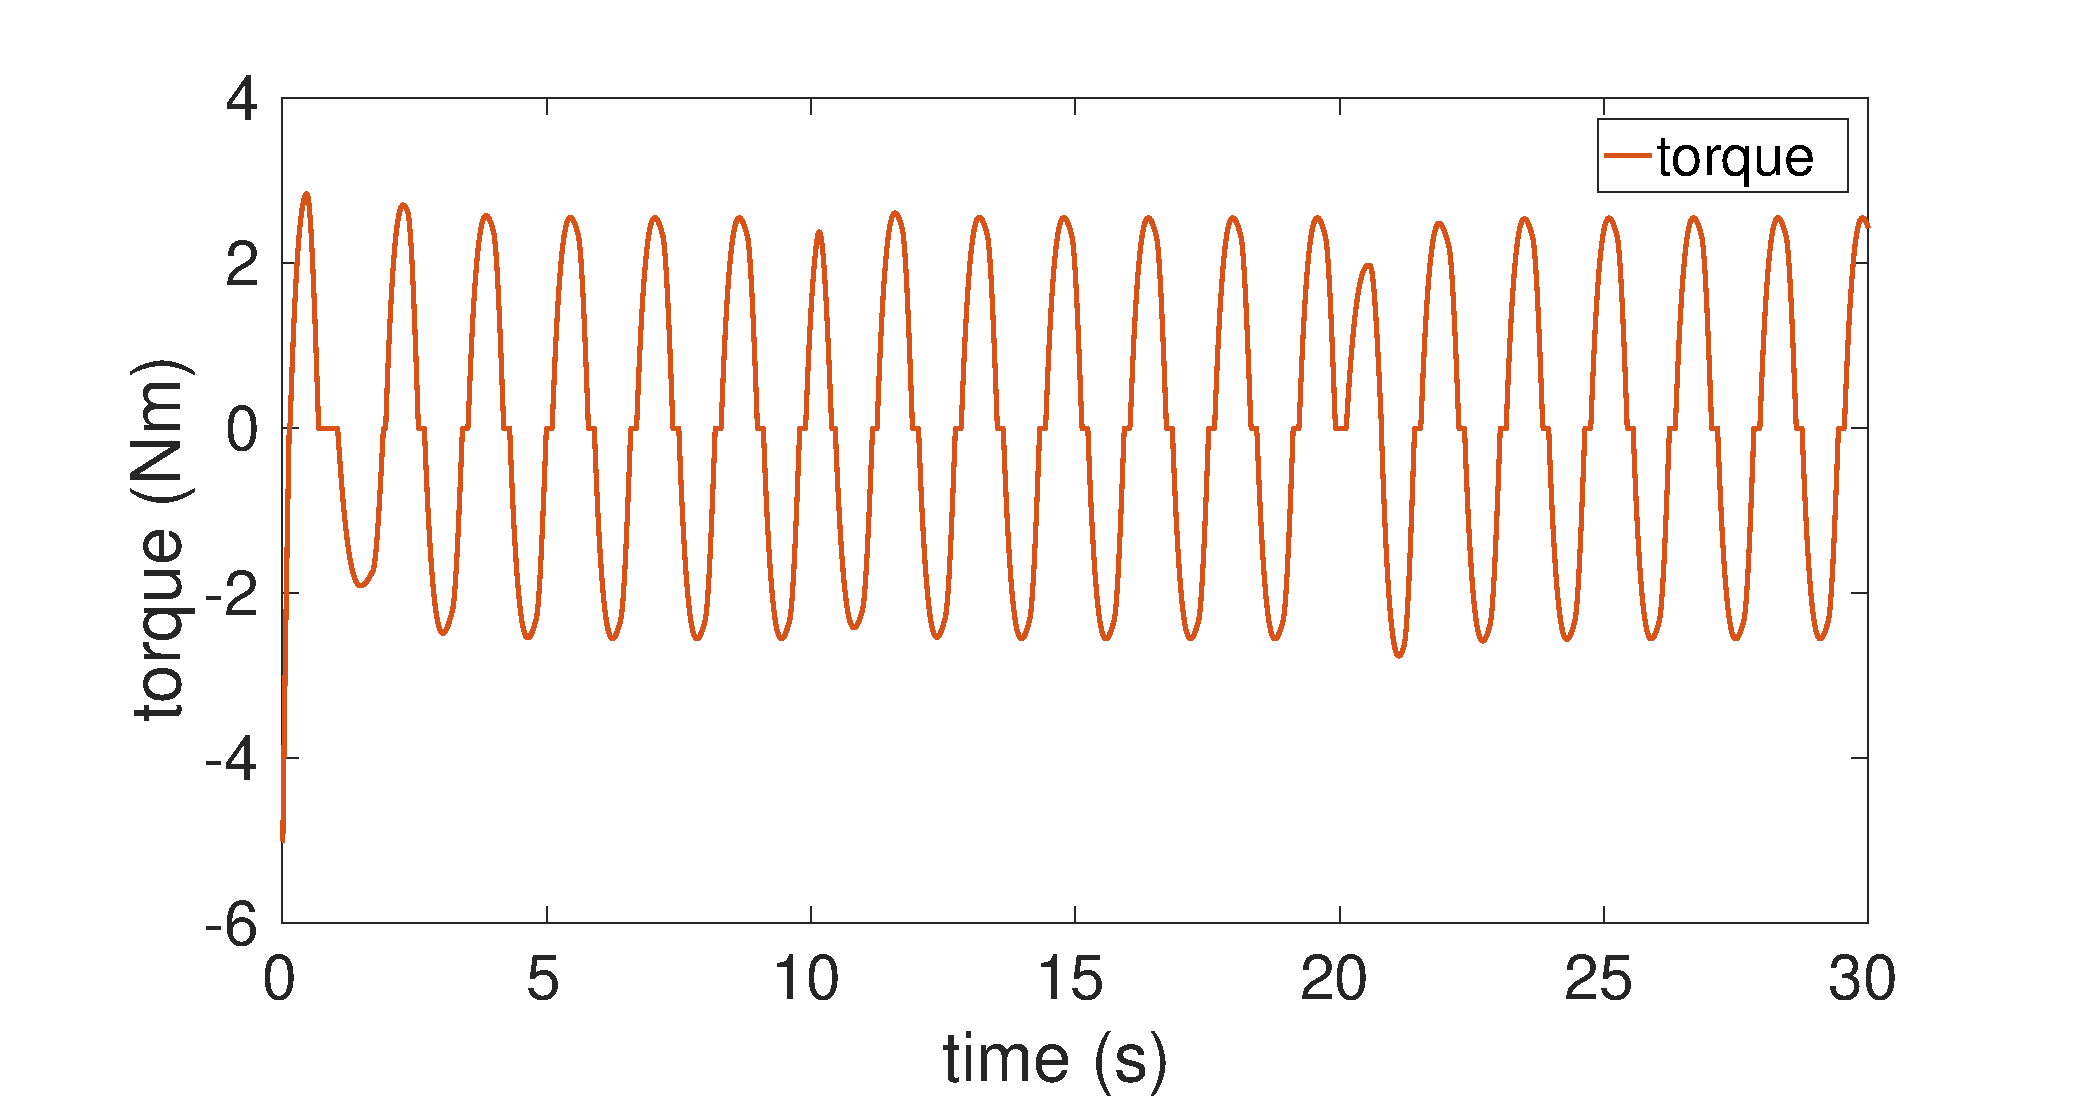
\includegraphics[scale=0.30]{figures/1-2-torque-for-change-average-position.eps}}
\subfigure[Joint position and average joint position]{\label{fig:a}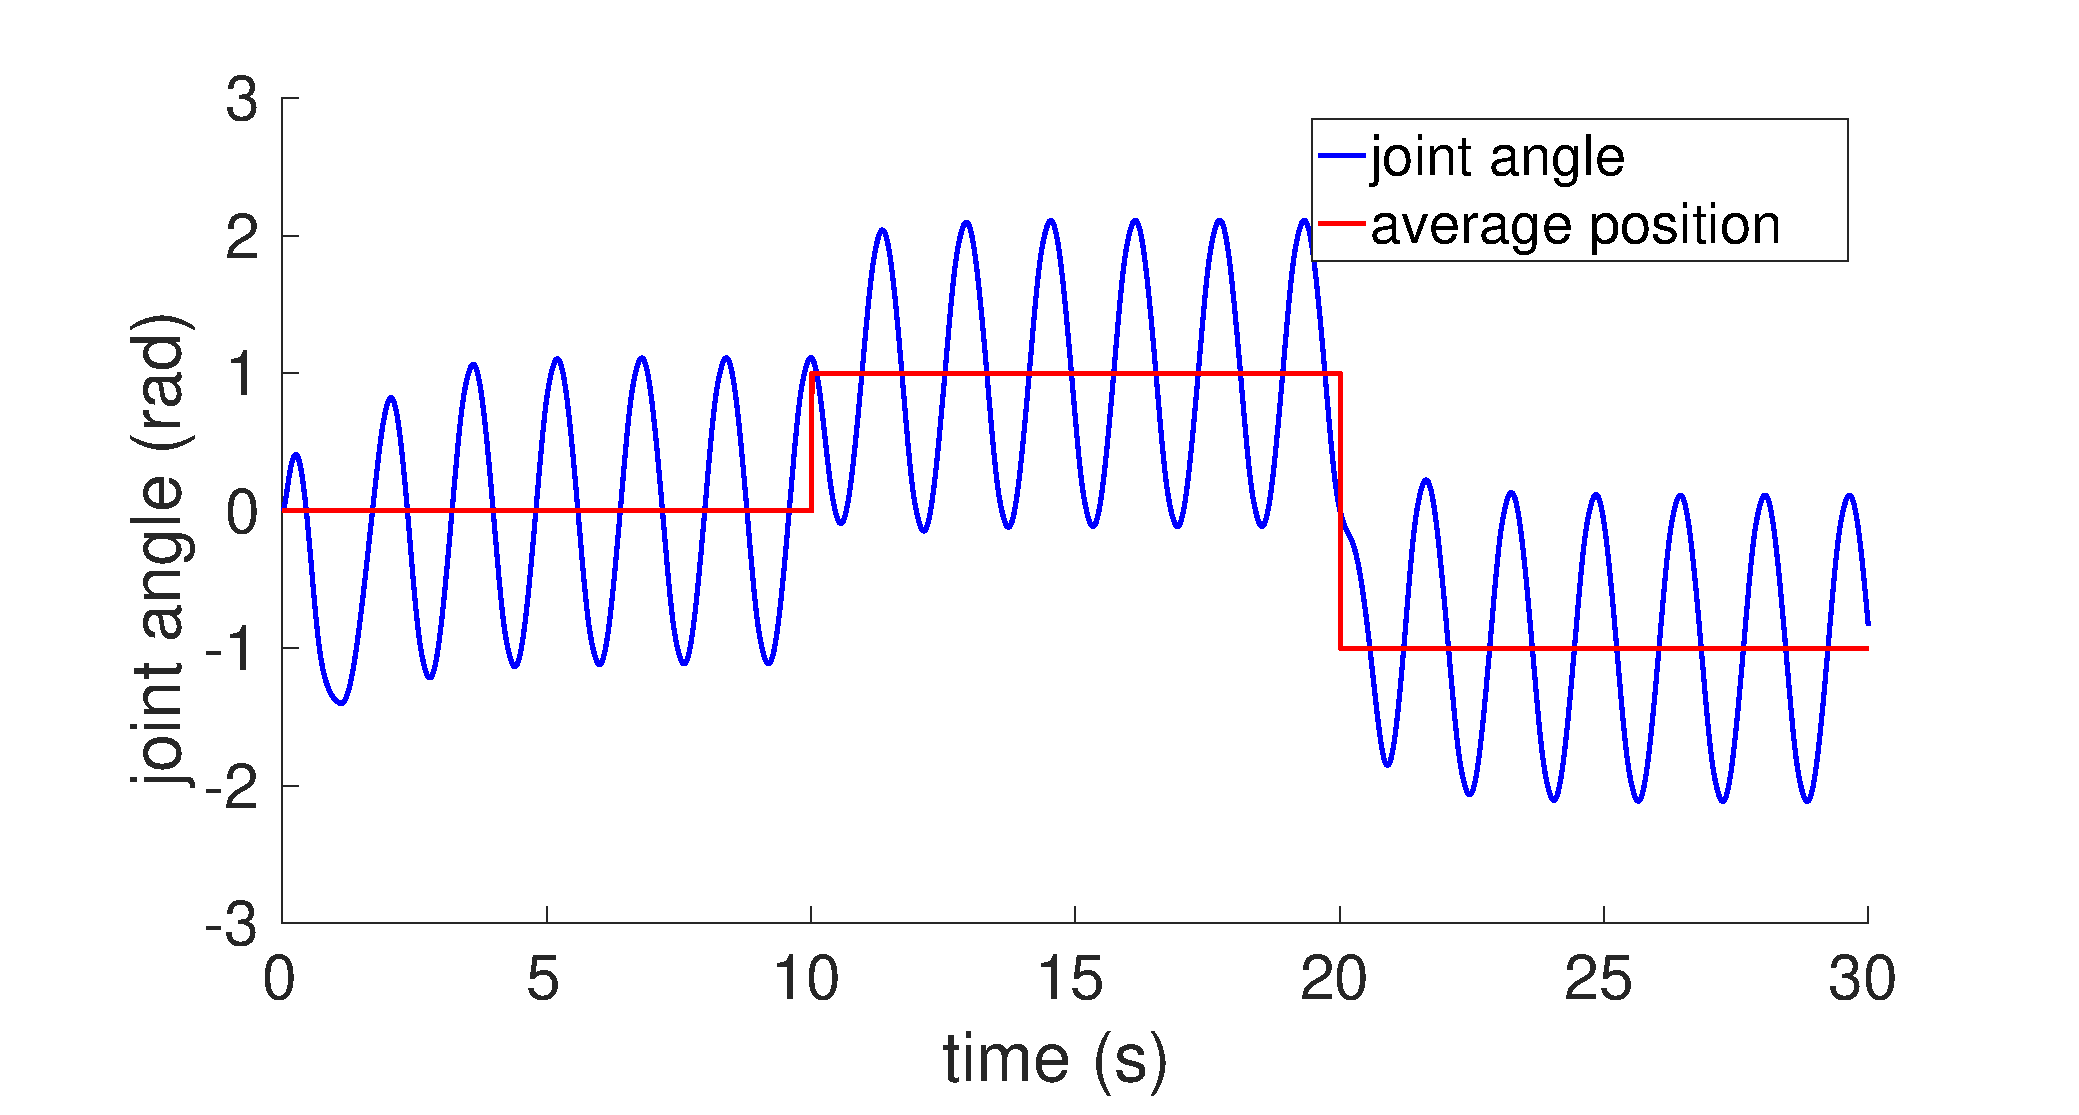
\includegraphics[scale=0.30]{figures/1-1-change-average-position.eps}}
\caption{Changing the average position of oscillation}
\label{fig:change-avg-pos}
\end{figure}

\subsection{Controlling the amplitude of the joint angle oscillations}
The tonic input to the oscillator is linearly related to the amplitude of the torque output and also approximately linearly to the amplitude of the position oscillations. Here the tonic input was linearly increased from 1.0 to 4.0 over 30 seconds, and as shown in figure \ref{fig:change-amp}, the amplitude of both the oscillations increases in a linear manner.

\begin{figure}[htbp]
\centering     %%% not \center
\subfigure[Torque output of the oscillator]{\label{fig:b}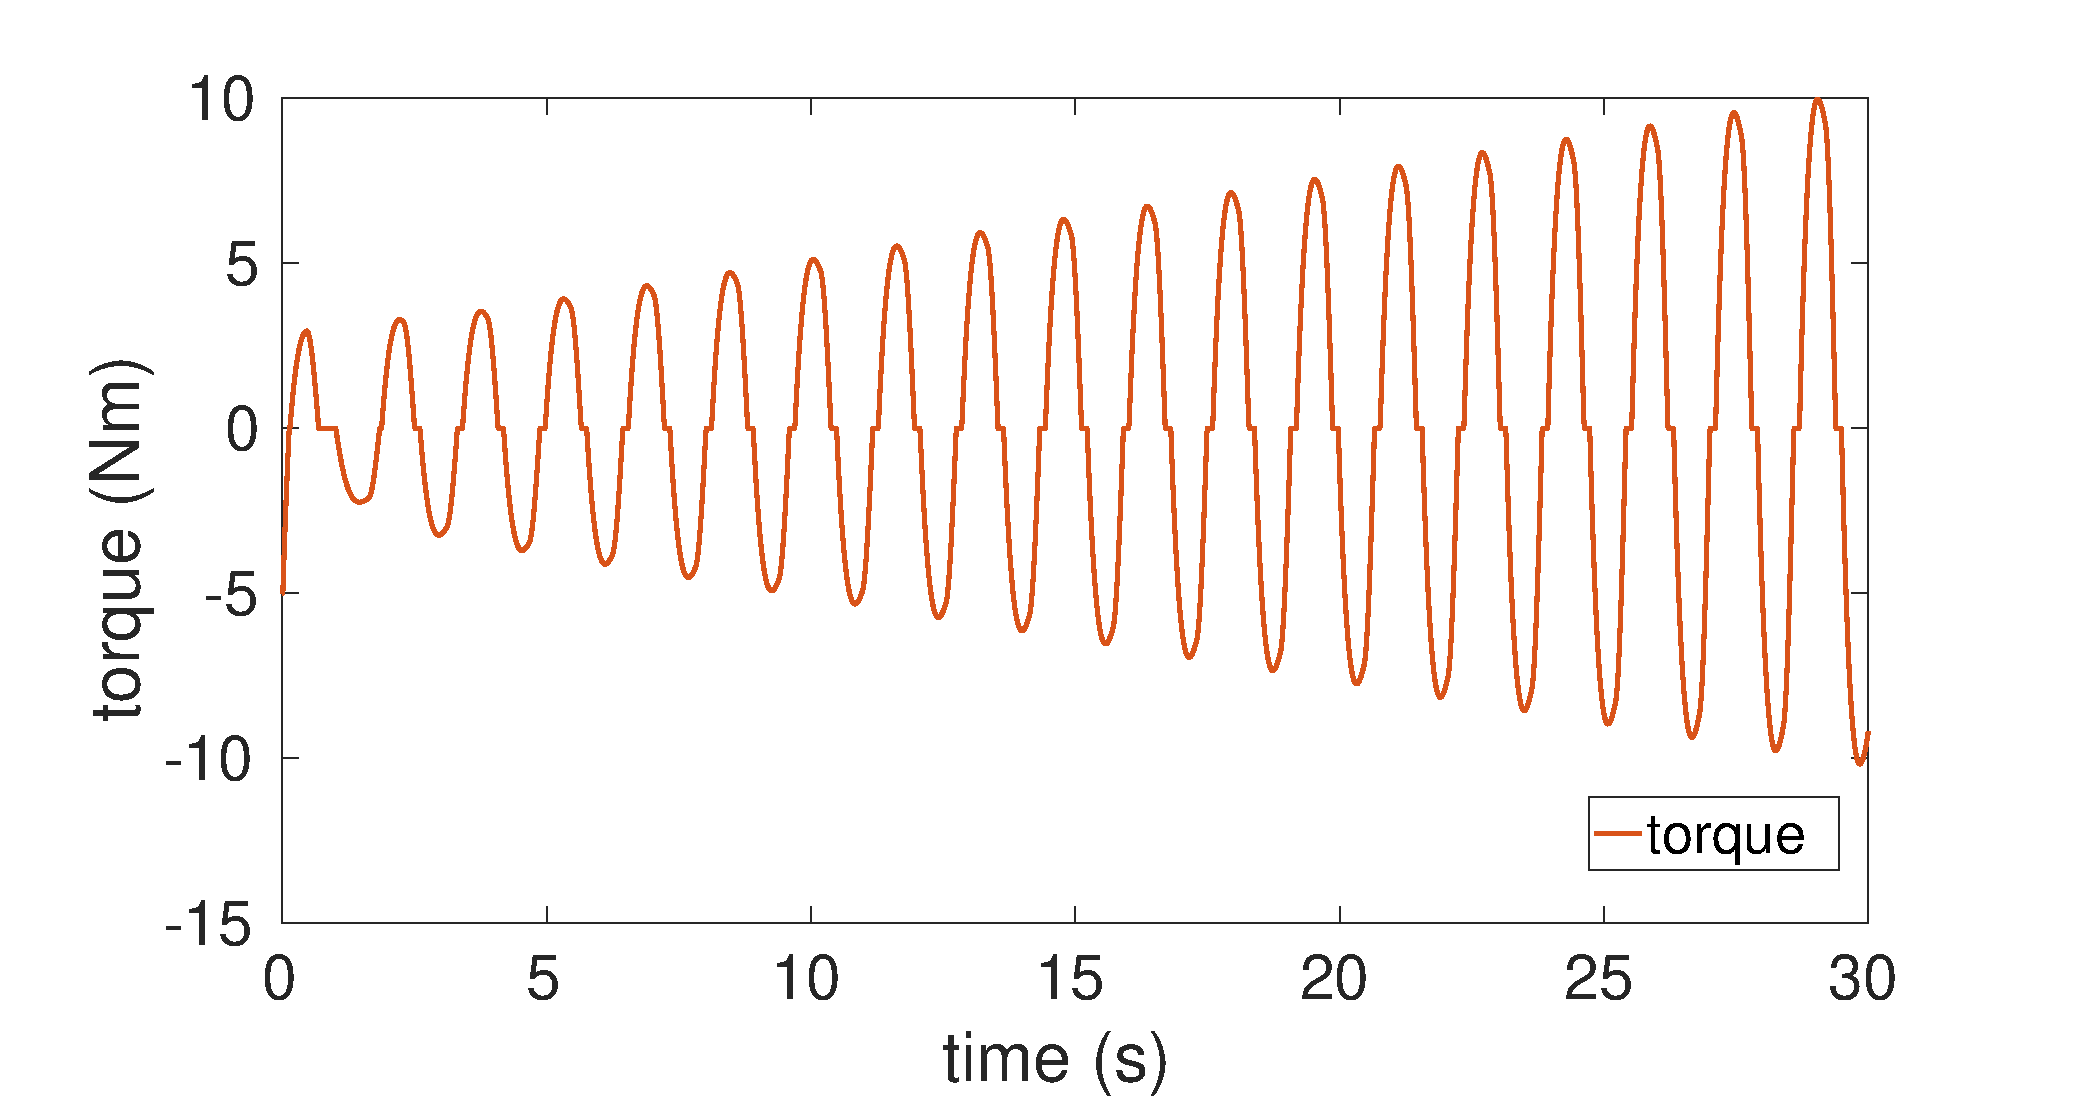
\includegraphics[scale=0.30]{figures/2-1-change-in-torque.eps}}
\subfigure[Joint position and average joint position]{\label{fig:a}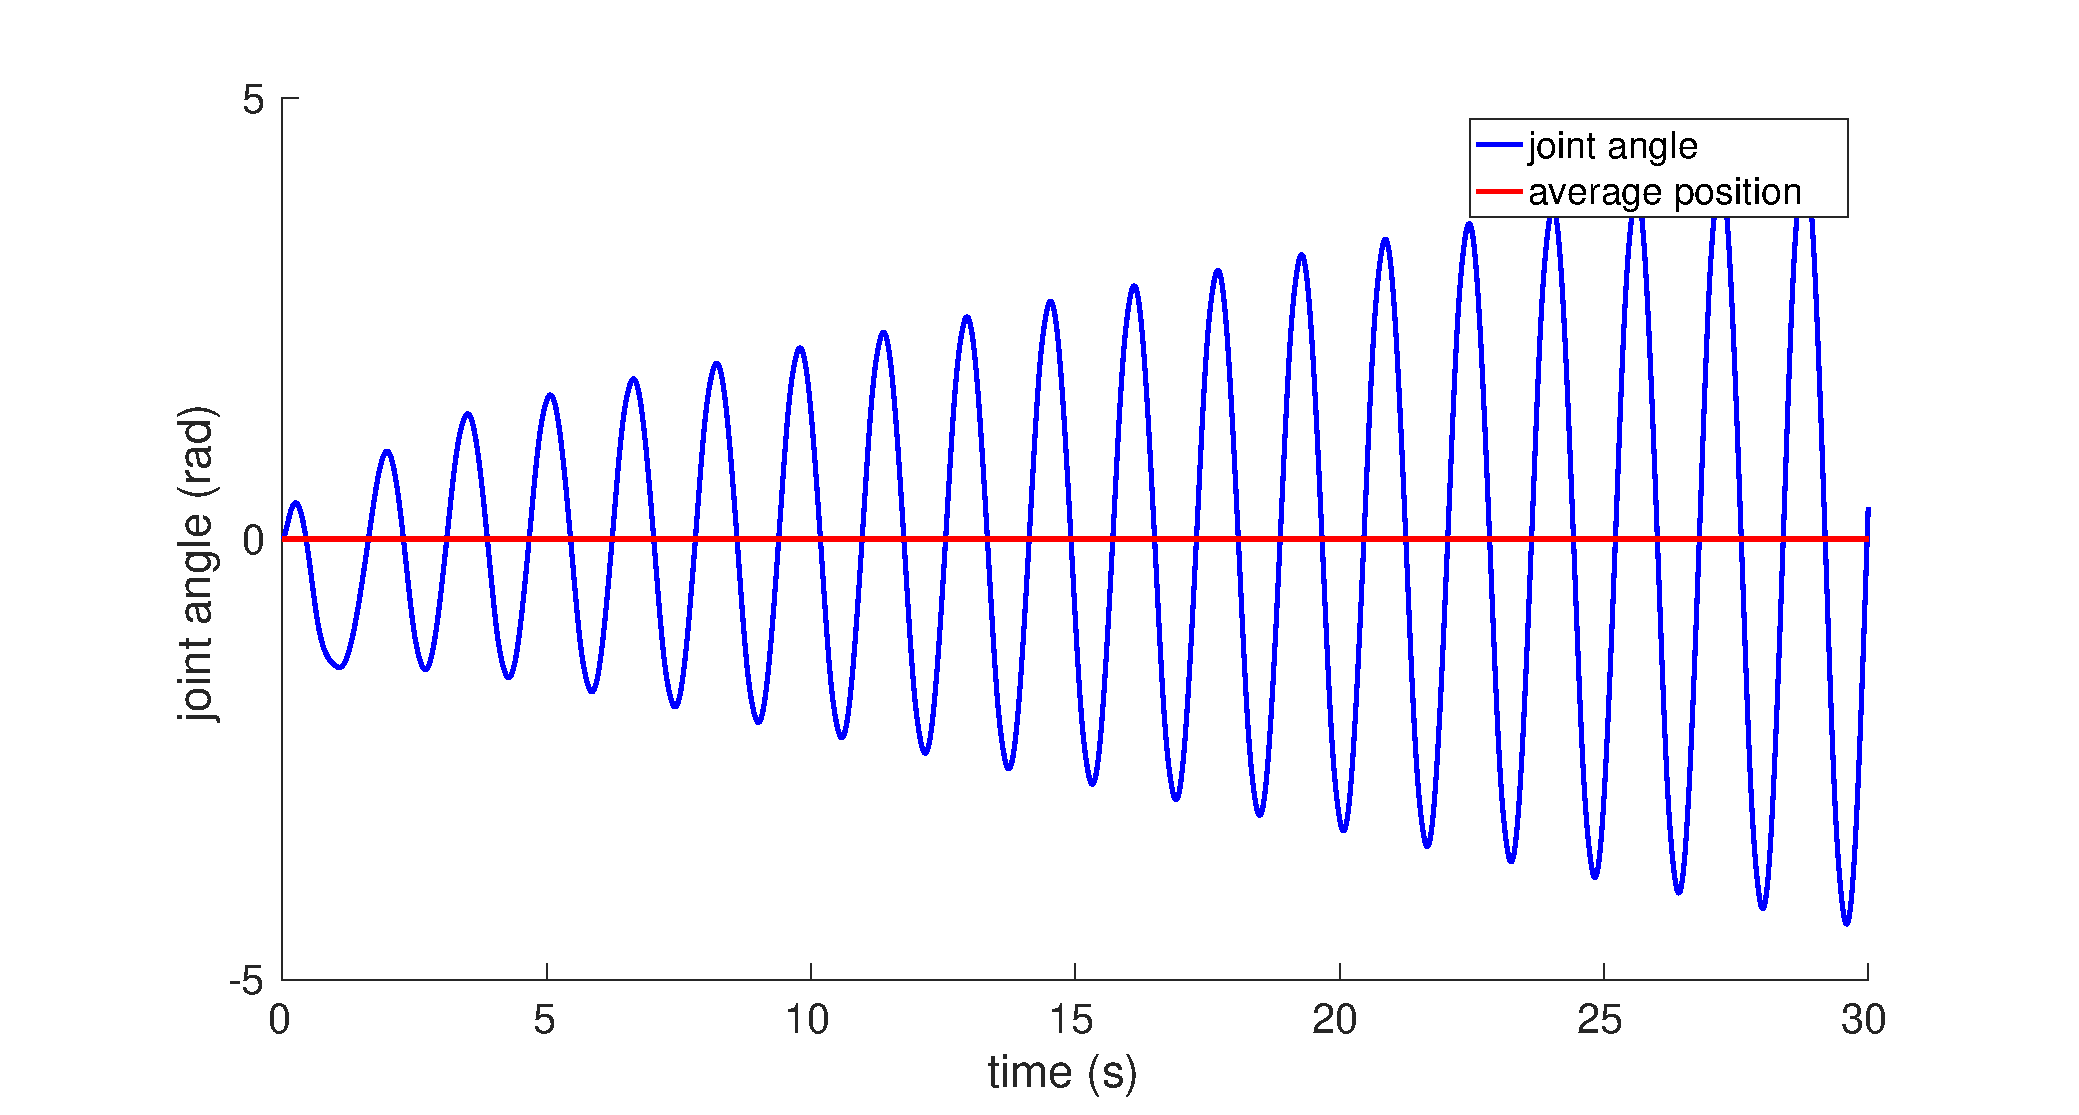
\includegraphics[scale=0.30]{figures/2-2-change-in-angle.eps}}
\subfigure[Tonic input to the oscillator]{\label{fig:b}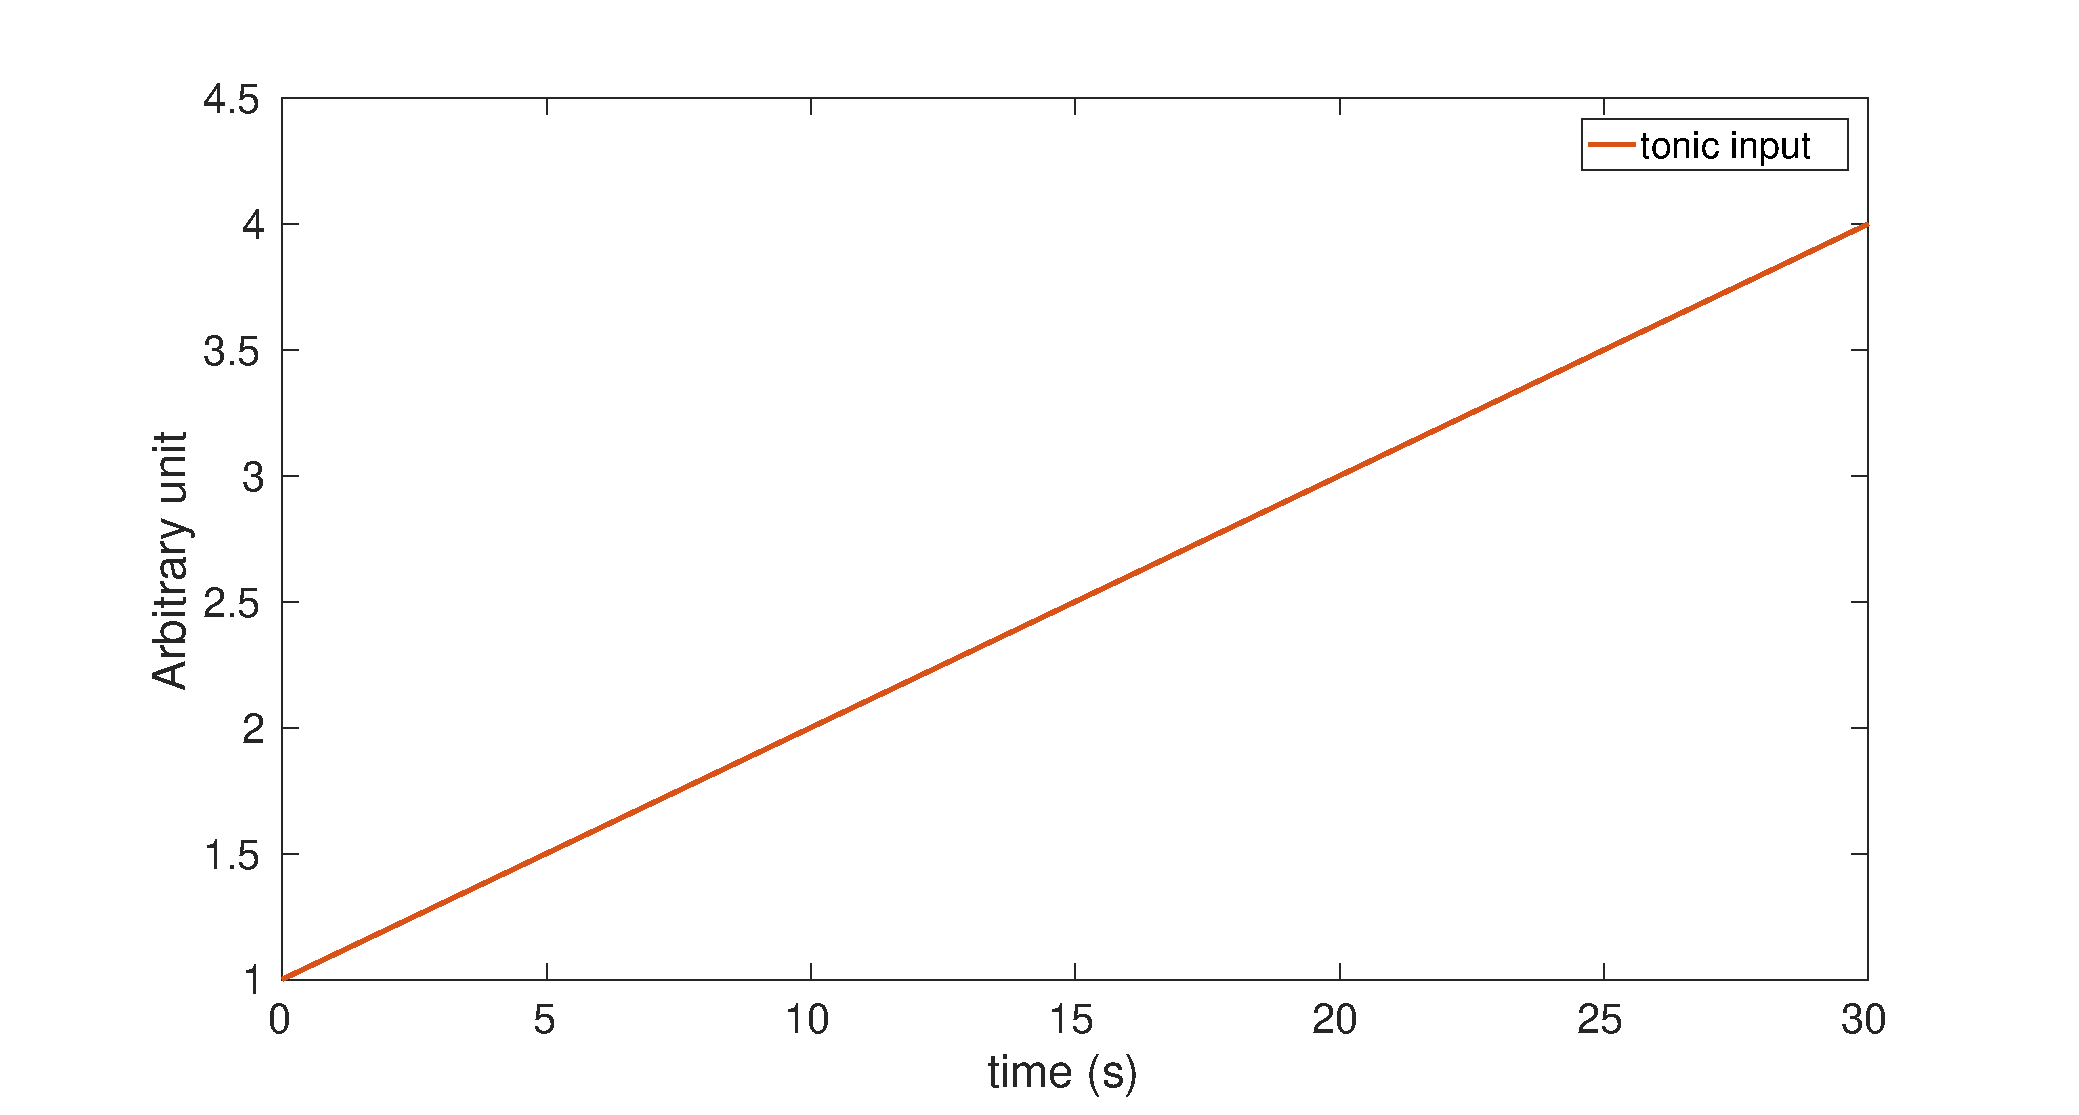
\includegraphics[scale=0.30]{figures/2-3-change-in-ut.eps}}
\caption{Changing the amplitude of oscillations}
\label{fig:change-amp}
\end{figure}

\subsection{Controlling the frequency of the joint angle oscillations}
By varying the time constants of the oscillator the frequency of the torque and joint angle oscillations can be varied. In figure \ref{fig:change-freq}, the time constant $t_1$ was set to 0.3 for the first 20 seconds, 0.6 for the next 20 seconds and to 0.9 for the last 20 seconds. The constant $t_2$ was set as $t_2 = 2.5 \times t_1$ as in \cite{ronsse2009computational}. As expected the frequency of both the torque and the joint angle oscillations decreases. However for the joint angles, the amplitude also increases as the frequency decreases. Throughout the 60 seconds, the tonic input $u_t$ was set to 1. Note that for both the 2 changes (at $t=20s$ and $t=40s$), the transitions were smooth.

\begin{figure}[htbp]
\centering     %%% not \center
\subfigure[Torque output of the oscillator]{\label{fig:b}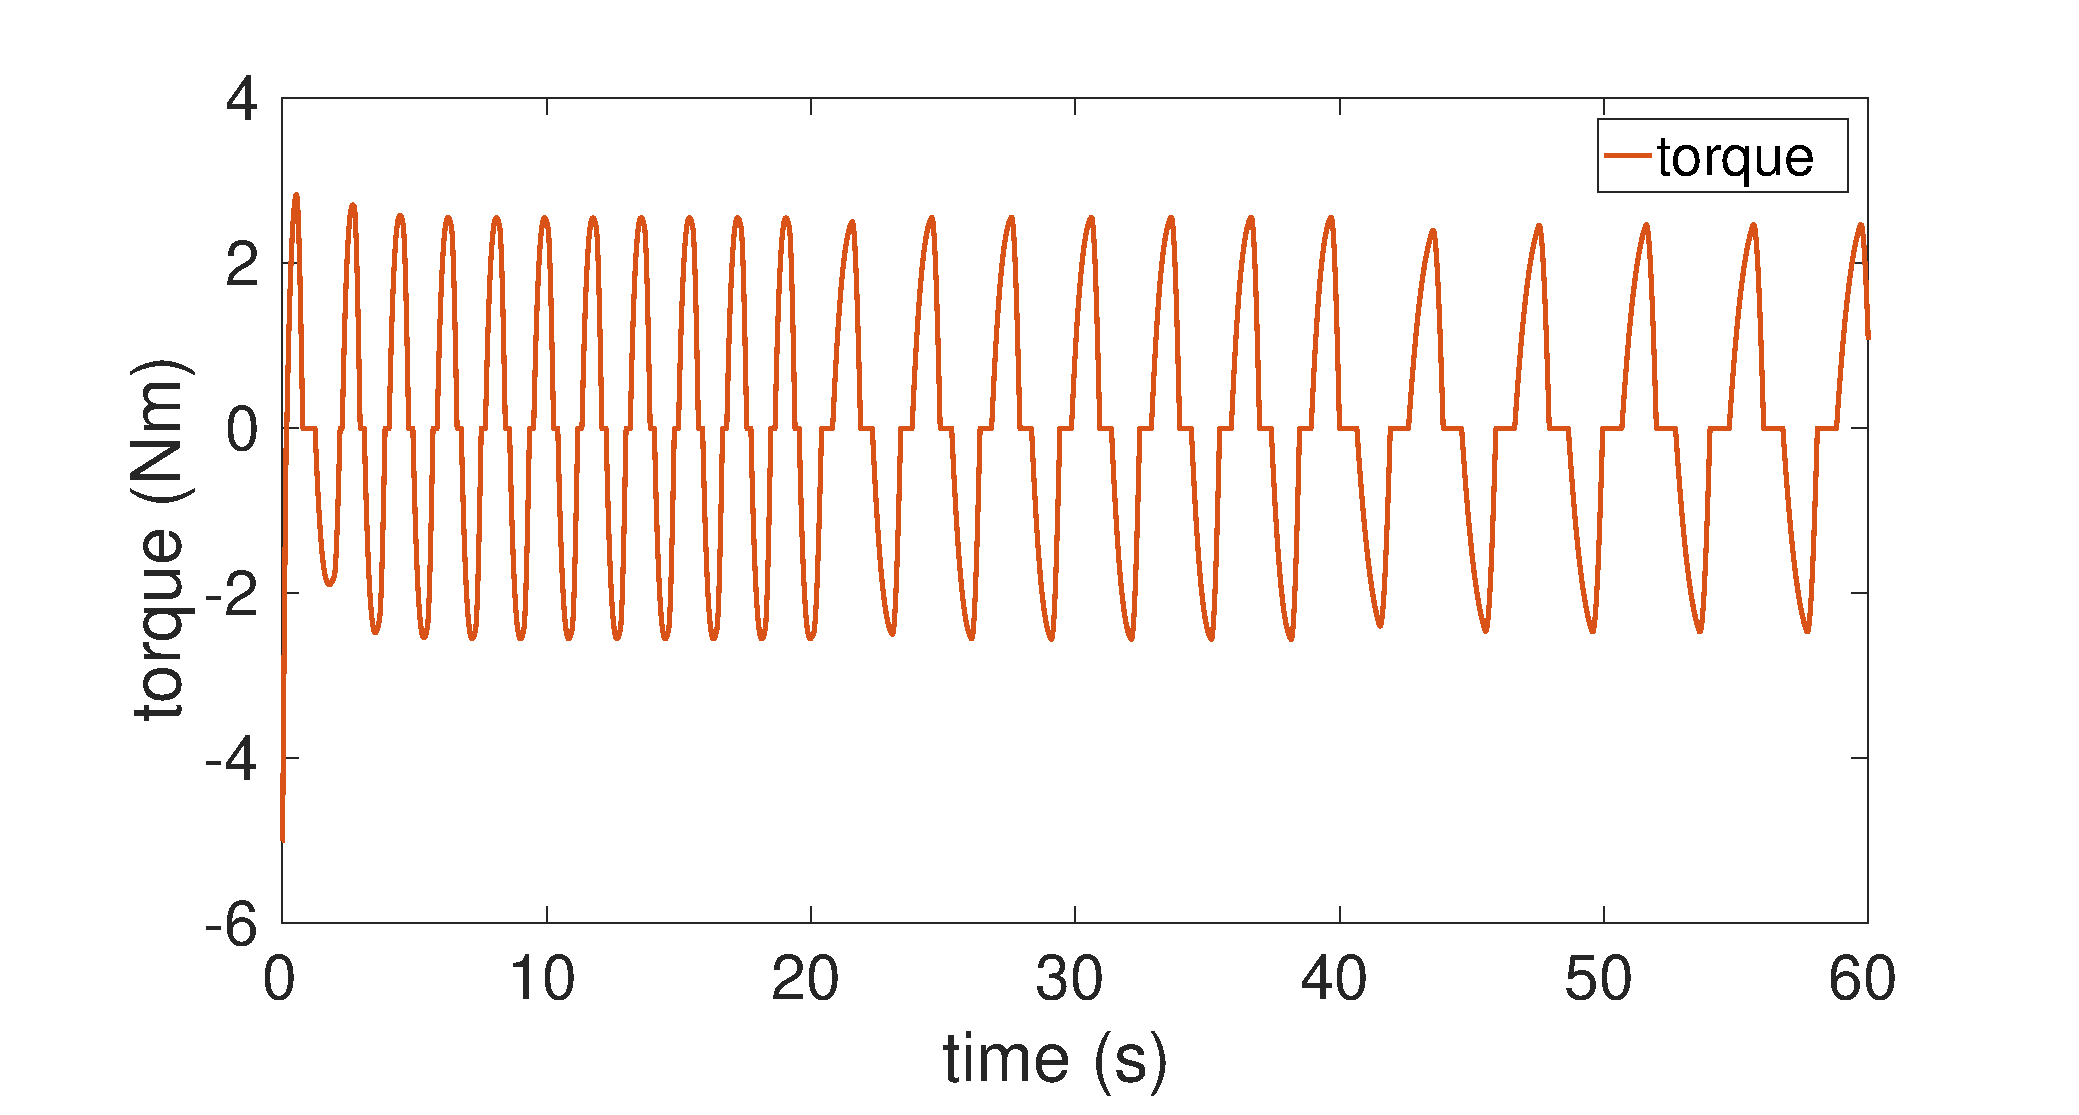
\includegraphics[scale=0.33]{figures/3-1-changing-freq-torque.eps}}
\subfigure[Joint position and average joint position]{\label{fig:a}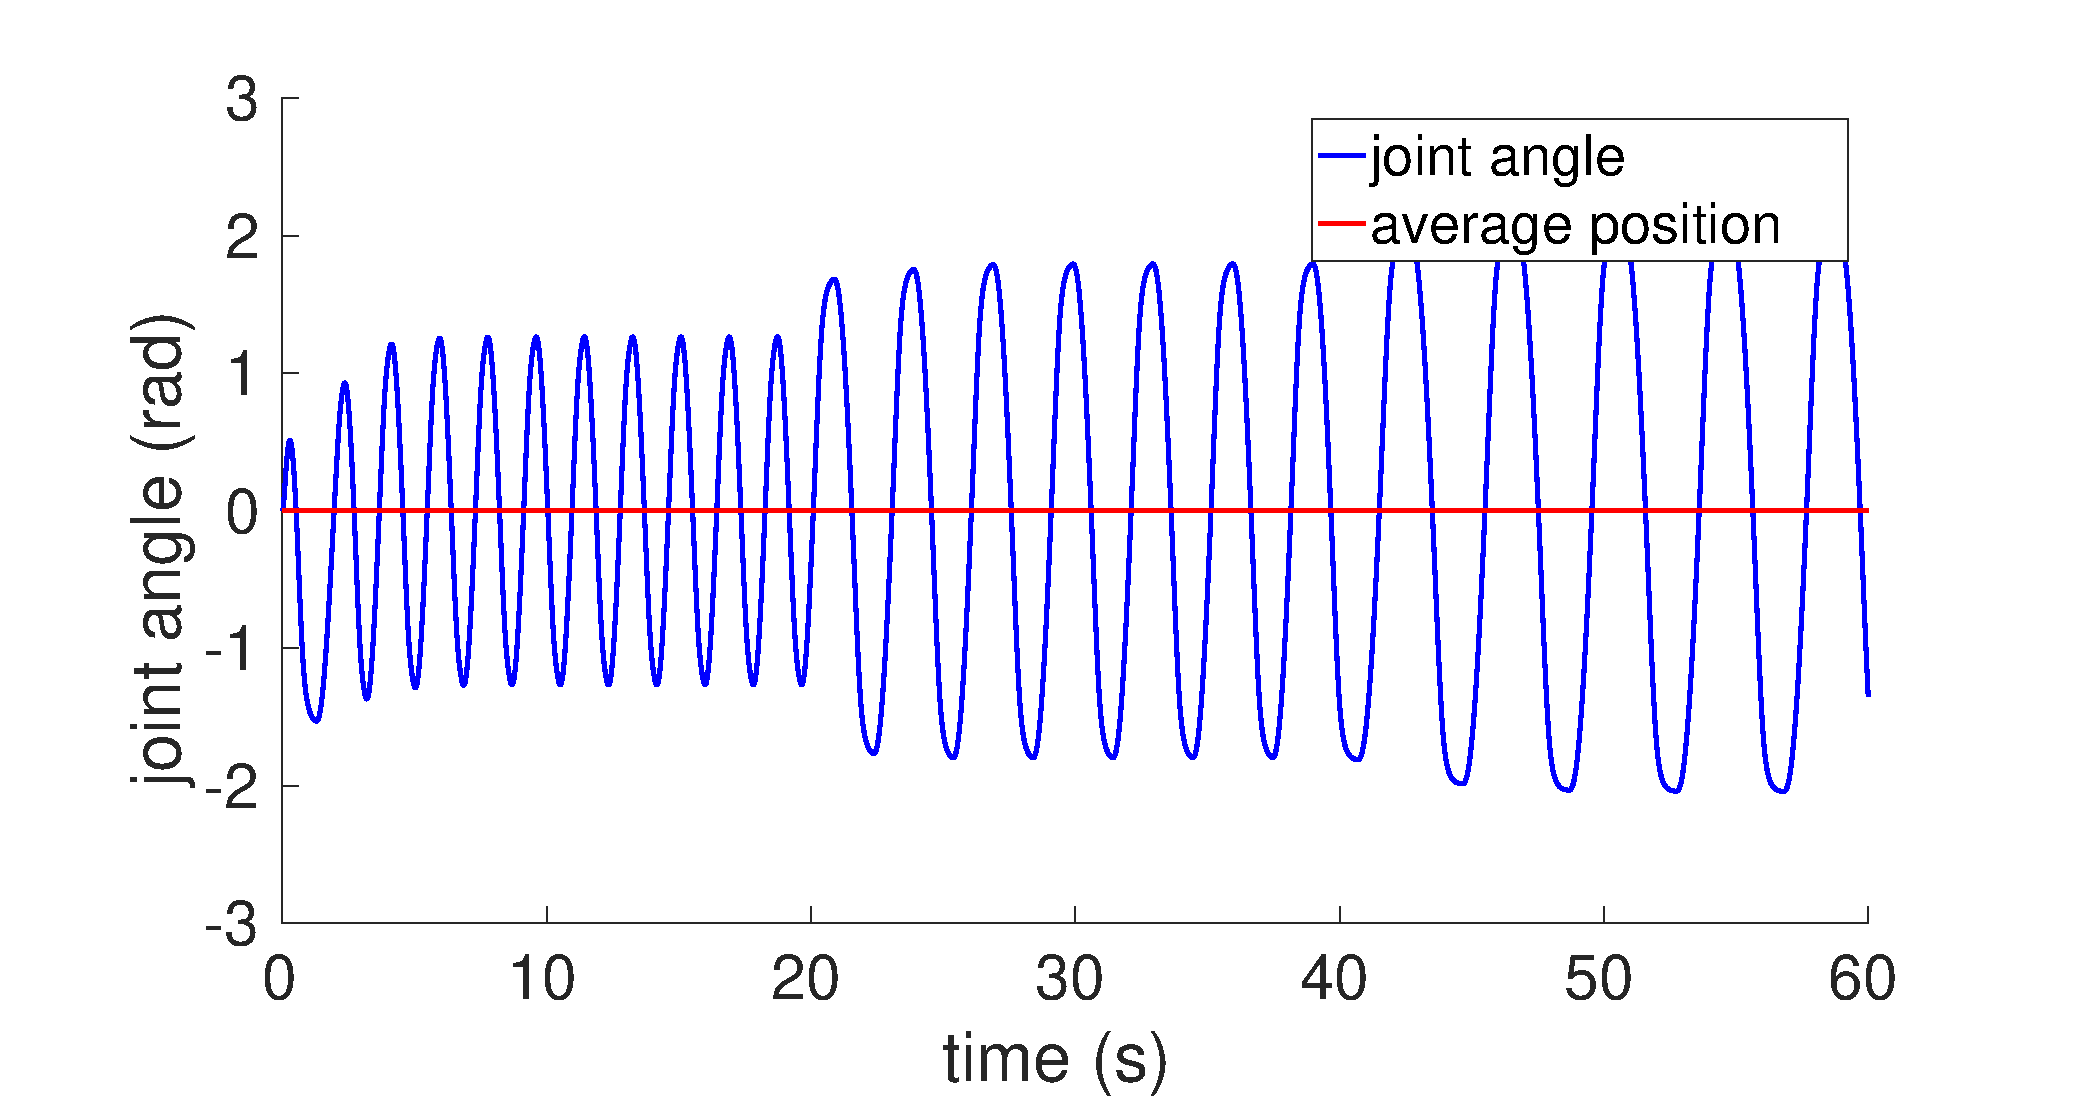
\includegraphics[scale=0.33]{figures/3-2-changing-freq-pos.eps}}
\caption{Changing the frequency of oscillation}
\label{fig:change-freq}
\end{figure}

\subsection{Anti-phase and in-phase oscillations}

\begin{figure}[htbp]
\centering     %%% not \center
\subfigure[Anti-phase oscillations]{\label{fig:b}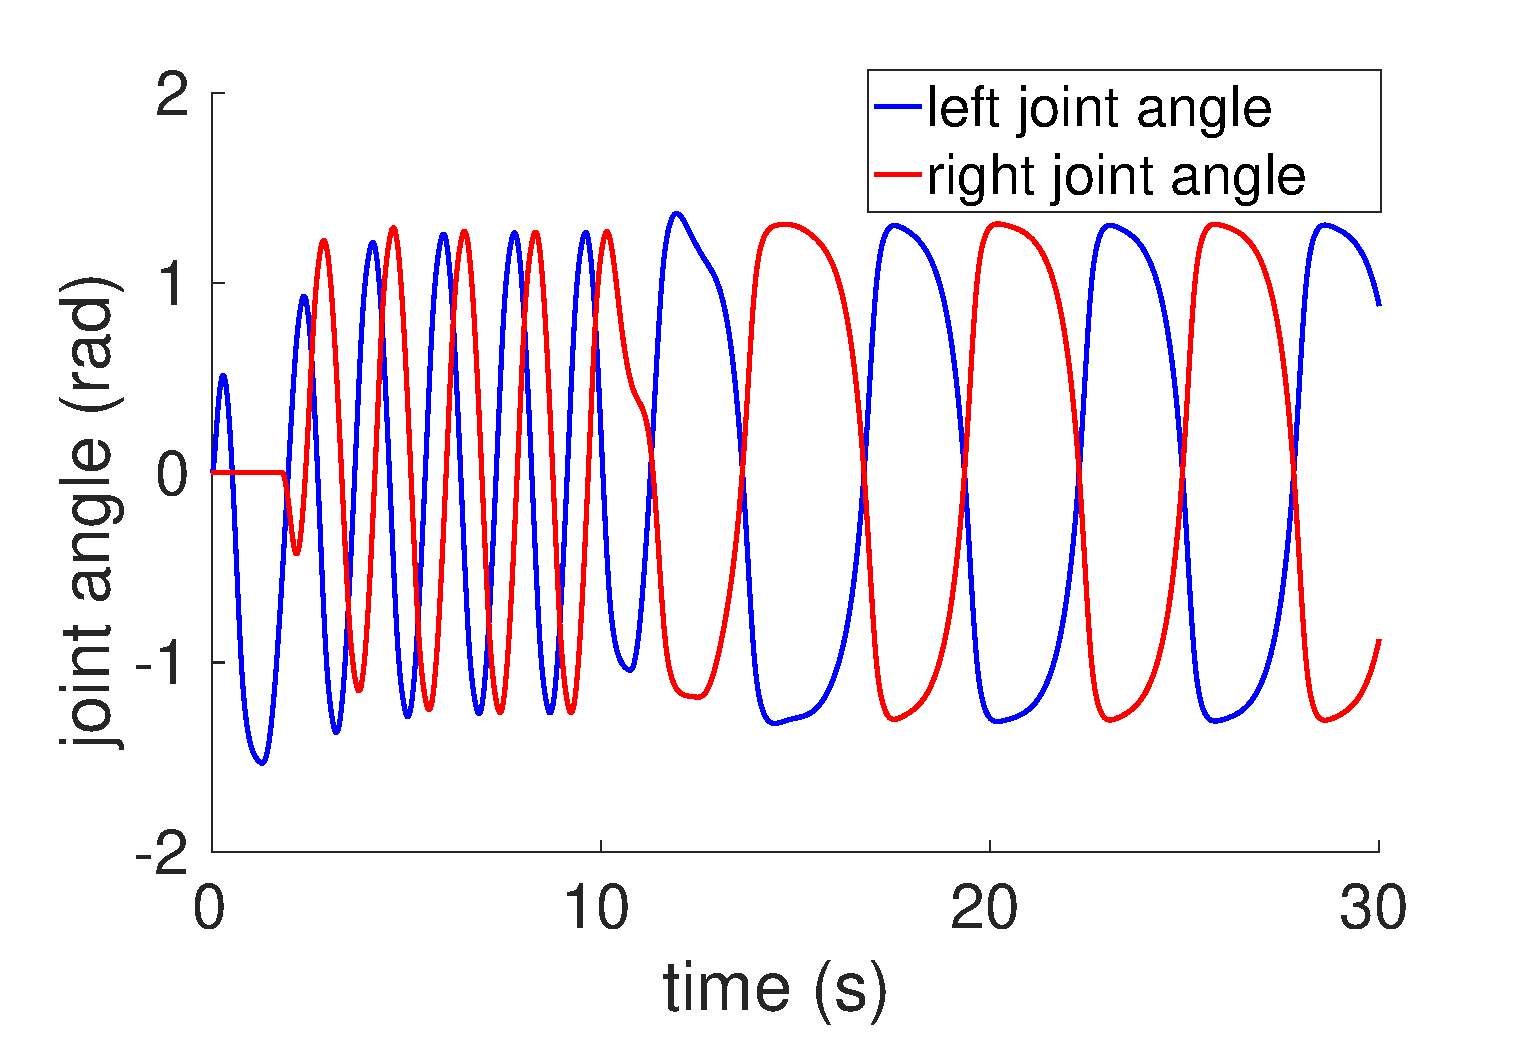
\includegraphics[scale=0.35]{figures/4-1-anti-phase.eps}}
\subfigure[In-phase oscillations]{\label{fig:a}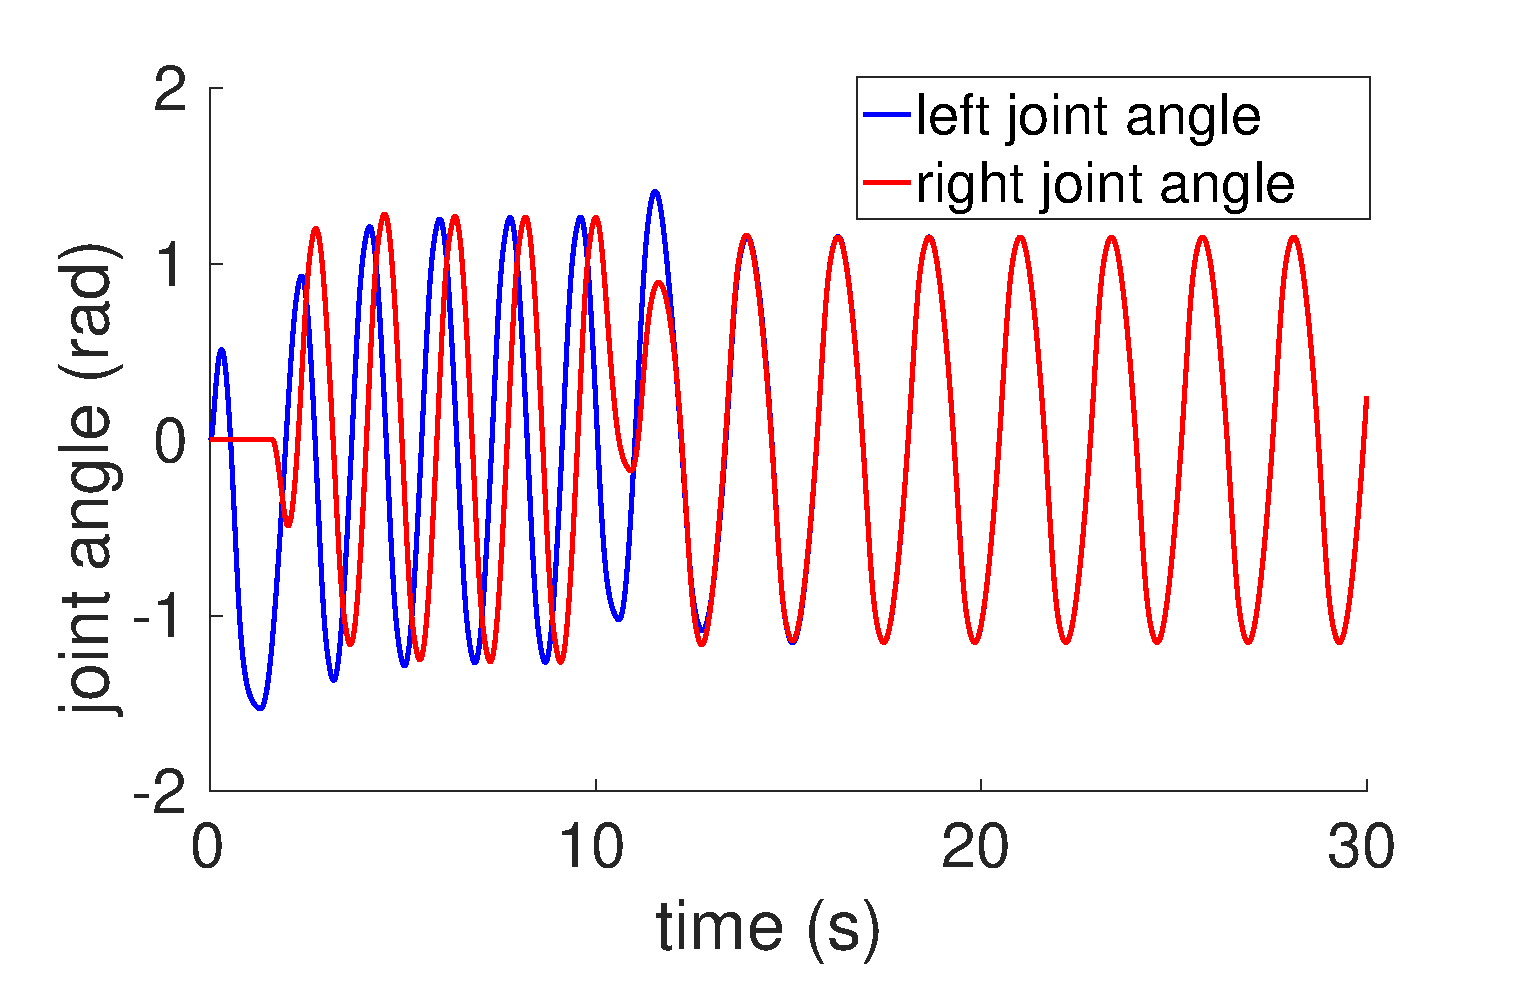
\includegraphics[scale=0.35]{figures/4-2-in-phase.eps}}
\caption{Anti-phase and in-phase oscillations}
\label{fig:in-anti-phase}
\end{figure}

\subsection{Stable attractors}



\begin{figure}[H]
\centering
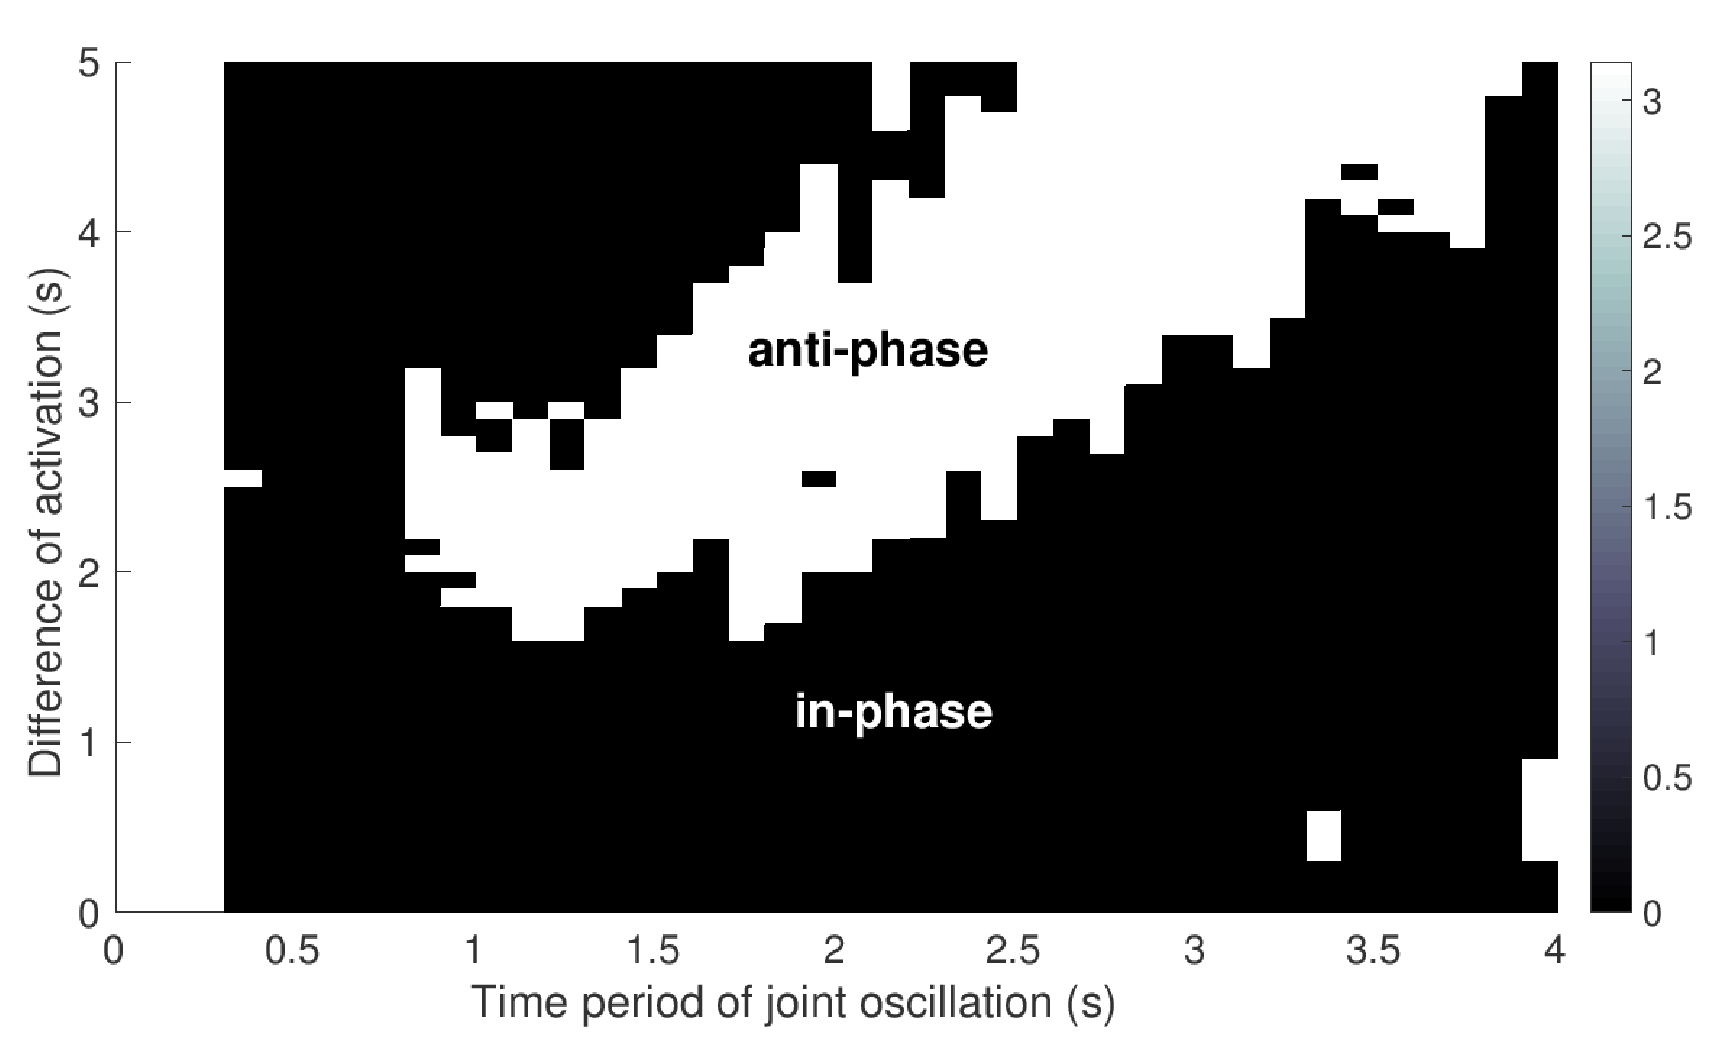
\includegraphics[scale=0.55]{figures/5-1-stable-attractors.eps}
\caption{Stable attractors for a broad range of time periods and initial phase difference between the two joints. As shown here, once the mutual coupling between the 2 joints is switched on, the joint oscillations converge to only 2 modes - either in-phase (0 phase difference) or anti-phase ($\pi$ phase difference).}
\label{fig:stable-attractors}
\end{figure}

\section{Coupled Oscillators}
\label{sec:Coupled_Oscillators}

\section{Robot Joint Control}
\label{sec:Robot_Joint_Control}

\section{Walk Optimization}
\label{sec:Walk_Optimization}

\section{Discussion}
\label{sec:Discussion}

\section{Future Work}
\label{sec:Future_Work}

\section{Conclusion}
\label{sec:Conclusion}

\cite{ronsse2009computational, williamson1998neural, matsuoka1987mechanisms, matsuoka1985sustained,Ishiguro2003}

%%%%%%%%%%%%%%%%%%%%%%%%%%%%%%%%%%%%%%
% hier werden - zum Ende des Textes - die bibliographischen Referenzen
% eingebunden
%
% Insbesondere stehen die eigentlichen Informationen in der Datei
% ``bib.bib''
%
\bibliographystyle{plain}
\bibliography{SA,primary}
\end{document}


